\lab{Interior Point 1: Linear Programs}{Interior Point 1: Linear Programs}

% Bold mu, lambda, and beta symbols for this lab. TODO: move to command.tex.
\def\Mu{\boldsymbol{\mu}}
\def\Lamb{\boldsymbol{\lambda}}
\def\Beta{\boldsymbol{\beta}}

\objective{For decades after its invention, the Simplex algorithm was the only competitive method for linear programming.
The past 30 years, however, have seen the discovery and widespread adoption of a new family of algorithms that rival--and in some cases outperform--the Simplex algorithm, collectively called \emph{Interior Point methods}.
One of the major shortcomings of the Simplex algorithm is that the number of steps required to solve the problem can grow exponentially with the size of the linear system.
Thus, for certain large linear programs, the Simplex algorithm is simply not viable.
Interior Point methods offer an alternative approach and enjoy much better theoretical convergence properties.
In this lab we implement an Interior Point method for linear programs, and in the next lab we will turn to the problem of solving quadratic programs.}

\section*{Introduction}

Recall that a linear program is a constrained optimization problem with a linear objective function and linear constraints.
The linear constraints define a set of allowable points called the \emph{feasible region}, the boundary of which forms a geometric object known as a \emph{polytope}.
The theory of convex optimization ensures that the optimal point for the objective function can be found among the vertices of the feasible polytope. The Simplex Method tests a sequence of such vertices until it finds
the optimal point.
Provided the linear program is neither unbounded nor infeasible, the algorithm is certain to produce the correct answer after a finite number of steps, but it does not guarantee an efficient path along the polytope toward the minimizer.
Interior point methods do away with the feasible polytope and instead generate a sequence of points that cut through the interior (or exterior) of the feasible region and converge iteratively to the optimal point.
Although it is computationally more expensive to compute such interior points, each step results in significant progress toward the minimizer.
See Figure \ref{fig:intPath} for an example of a path using an Interior Point algorithm.
In general, the Simplex Method requires many more iterations (though each iteration is less expensive computationally).

\begin{figure}
\centering
\includegraphics[width=\textwidth]{figures/interiorPath.pdf}
\caption{A path traced by an Interior Point algorithm.}
\label{fig:intPath}
\end{figure}

\section*{Primal-Dual Interior Point Methods} % ALGORITHM =====================
Some of the most popular and successful types of Interior Point methods are known as Primal-Dual Interior Point methods.
Consider the following linear program:
\begin{align*}
\text{minimize }\qquad &\c\trp \x\\
\text{subject to }\qquad &A\x = \b\\
&\x \succeq \0.
\end{align*}
Here, $\x, \c \in \mathbb{R}^n$, $\b \in \mathbb{R}^m$, and $A\in\mathbb{R}^{m\times n}$ with full row rank.
% By $x \succeq 0$, we simply mean that each coordinate of $x$ is nonnegative.
% Note that this formulation is quite general, as any linear program can be posed in this manner, after appropriate transformations.
This is the \emph{primal} problem, and its \emph{dual} takes the form:
\begin{align*}
\text{maximize }\qquad &\b\trp \Lamb\\
\text{subject to }\qquad &A\trp \Lamb + \Mu = \c\\
&\Mu,\Lamb \succeq \0,
\end{align*}
where $\Lamb \in \mathbb{R}^m$ and $\Mu \in \mathbb{R}^n$.
% Changed s to \mu to match the textbook.

\subsection*{KKT Conditions}

The theory of convex optimization gives us necessary and sufficient conditions for the solutions to the primal and dual problems via the Karush-Kuhn-Tucker (KKT) conditions.
The Lagrangian for the primal problem is as follows:
\[
\CalL(\x, \Lamb, \Mu)
= \c\trp \x + \Lamb\trp (\b - A\x) - \Mu\trp \x
\]
The KKT conditions are
\begin{align*}
A\trp \Lamb + \Mu &= \c\\
A\x &= \b\\
x_i\mu_i &= 0, \quad i = 1,2,\ldots,n,\\
\x, \Mu &\succeq 0.
\end{align*}
It is convenient to write these conditions in a more compact manner, by defining an almost-linear function $F$ and setting it equal to zero:
\begin{align*}
F(\x,\Lamb,\Mu) :=
\begin{bmatrix}
A\trp \Lamb + \Mu - \c\\
A\x - \b\\
M\x\\
\end{bmatrix}
&= \0,\\
(\x,\Mu &\succeq \0),
\end{align*}
where $M = \text{diag}(\mu_1,\mu_2,\ldots,\mu_n)$.
Note that the first row of $F$ is the KKT condition for dual feasibility, the second row of $F$ is the KKT condition for the primal problem, and the last row of $F$ accounts for complementary slackness.

\begin{comment} % Derivation overkill vvvvvvvvvvvvvvvvvvvvvvvvvvvvvvvvvvvvvvvvv
First, we calculate the so-called \emph{Lagrangian function} for our linear program.
Recall that the Lagrangian function for a general constrained optimization problem of the form
\begin{align*}
\text{minimize }\qquad &f(x)\\
\text{subject to }\qquad &c_i(x) = 0, \quad i = 1,2,\ldots,k,\\
&d_i(x) \geq 0, \quad i = 1,2,\ldots,j,
\end{align*}
is defined to be
\[
\mathcal{L}(x, \lambda, s) := f(x) - \displaystyle\sum_{i=1}^k\lambda_ic_i(x) - \displaystyle\sum_{i=1}^js_id_i(x).
\]
From here, the KKT conditions are
\begin{align*}
\nabla_x\mathcal{L}(x,\lambda,s) &= 0,\\
c_i(x) &= 0,\quad i = 1,2,\ldots,k,\\
s_id_i(x) &= 0,\quad i=1,2,\ldots,j,\\
d_i(x) &\geq 0,\quad i=1,2,\ldots,j,\\
s_i &\geq 0,\quad i=1,2,\ldots,j.
\end{align*}
For our linear program, $f(x) = c\trp x$, $c_i(x) = A_i\trp x - b_i$ (where $A_i$ denotes the $i$-th row of $A$), and $d_i(x) = x_i$.
Hence, you can check that our Lagrangian function is
\[
\mathcal{L}(x,\lambda,s) = c\trp x - \lambda\trp (Ax - b) - s\trp x.
\]
We then calculate
\[
\nabla_x\mathcal{L}(x,\lambda,s) = (c\trp  - \lambda\trp A - s\trp )\trp  = c - A\trp \lambda - s.
\]
The KKT conditions can now be expressed as follows:
\begin{align*}
A\trp \lambda + s &= c\\
A\x &= \b\\
x_is_i &= 0, \quad i = 1,2,\ldots,n,\\
\x, \mathbf{s} &\succeq 0.
\end{align*}
In fact, it is convenient to write these conditions in a more compact manner, by defining an almost-linear function $F$ and setting it equal to zero:
\begin{align*}
F(\x,\Lamb,\Mu) :=
\begin{bmatrix}
A\trp \lambda + s - c\\
Ax - b\\
XSe\\
\end{bmatrix}
&= 0,\\
(\x,\mathbf{s} &\succeq \0),
\end{align*}
where $X = \text{diag}(x_1,x_2,\ldots,x_n)$, $S = \text{diag}(s_1,s_2,\ldots,s_n)$, and $e = (1,1,\ldots,1)\trp $.
\end{comment} % Derivation overkil ^^^^^^^^^^^^^^^^^^^^^^^^^^^^^^^^^^^^^^^^^^^^

\begin{problem} % First step: define F(x,lamb,mu) -----------------------------
Define a function \li{interiorPoint()} that will be used to solve the complete interior point problem.
This function should accept $A$, $\b$, and $\c$ as parameters, along with the keyword arguments \li{niter=20} and \li{tol=1e-16}.
The keyword arguments will be used in a later problem.

In the next few problems, you will be writing functions within this function to solve the interior point problem one step at a time.

For this problem, within the \li{interiorPoint()} function, write a function for the vector-valued function $F$ described above.
This function should accept $\x$, $\Lamb$, and $\Mu$ as parameters and return a 1-dimensional NumPy array with $2n+m$ entries.
\end{problem}

\subsection*{Search Direction}

A Primal-Dual Interior Point method is a line search method that starts with an initial guess $(\x_0\trp , \Lamb_0\trp , \Mu_0\trp )$ and produces a sequence of points that converge to $({\x^*}\trp , {\Lamb^*}\trp , {\Mu^*}\trp )$, the solution to the KKT equations and hence the solution to the original linear program.
%We now describe how to select the search direction and step length at each iteration of the algorithm.
The constraints on the problem make finding a search direction and step length a little more complicated than for the unconstrained line search we have studied previously.

In the spirit of Newton's Method, we can form a linear approximation of the system $F(\x,\Lamb,\Mu) = \0$ centered around our current point $(\x, \Lamb, \Mu)$, and calculate the direction $(\triangle \x\trp , \triangle \Lamb\trp , \triangle \Mu\trp )$ in which to step to set the linear approximation equal to $\0$.
This equates to solving the linear system:
\begin{align}
DF(\x,\Lamb,\Mu)
\begin{bmatrix}\triangle \x\\ \triangle \Lamb\\ \triangle \Mu\end{bmatrix}
= - F(\x,\Lamb,\Mu) \label{eq:naiveNewton}
\end{align}
Here $DF(\x,\Lamb,\Mu)$ denotes the total derivative matrix of $F$.
We can calculate this matrix block-wise by obtaining the partial derivatives of each block entry of $F(\x,\Lamb, \Mu)$ with respect to $\x$, $\Lamb$, and $\Mu$, respectively.
We thus obtain:
\[
DF(\x,\Lamb,\Mu) = \left[\begin{array}{ccc}
0 & A\trp  & I \\
A & 0 & 0 \\
M & 0 & X
\end{array}\right]
\]
where $X = \text{diag}(x_1,x_2,\ldots,x_n).$

\begin{comment} % More derivation overkill vvvvvvvvvvvvvvvvvvvvvvvvvvvvvvvvvvvv
For example, consider the topmost block entry of $F(\x,\Lamb,\Mu)$, given by
\[
A\trp \lambda + s - c.
\]
We calculate the partial derivatives of this expressions as follows:
\begin{align*}
\frac{\partial}{\partial x}[A\trp \lambda + s - c] &= 0,\\
\frac{\partial}{\partial \lambda}[A\trp \lambda + s - c] &= A\trp ,\\
\frac{\partial}{\partial s}[A\trp \lambda + s - c] &= I.\\
\end{align*}
Hence, the topmost block row of $DF(\x,\Lamb,\Mu)$ is given by
\[
\begin{bmatrix}
0 \quad A\trp  \quad I\\
\end{bmatrix}.
\]
Continuing in this manner, we can calculate the entire derivative matrix, which leads us to the following linear system:
\end{comment} % More derivation overkill ^^^^^^^^^^^^^^^^^^^^^^^^^^^^^^^^^^^^^^

Unfortunately, solving Equation \ref{eq:naiveNewton} often leads to a search direction that is too greedy.
Even small steps in this direction may lead the iteration out of the feasible region by violating one of the constraints.
To remedy this, we define the \emph{duality measure} $\nu$\footnote{$\nu$ is the Greek letter for $n$, pronounced ``nu.''} of the problem: \[\nu = \frac{\x\trp \Mu}{n} \]
The idea is to use Newton's method to identify a direction that strictly decreases $\nu$.
Thus instead of solving Equation \ref{eq:naiveNewton}, we solve:
\begin{align}
DF(\x,\Lamb,\Mu)
\begin{bmatrix}\triangle \x\\ \triangle \Lamb\\ \triangle \Mu\end{bmatrix}
= - F(\x,\Lamb,\Mu) +
\begin{bmatrix} \0 \\ \0 \\ \sigma\nu\e \end{bmatrix}
\label{eq:newNewton}
\end{align}
where $\e = (1,1,\ldots,1)\trp $ and $\sigma \in [0,1)$ is called the \emph{centering parameter}.
The closer $\sigma$ is to 0, the more similar the resulting direction will be to the plain Newton direction.
The closer $\sigma$ is to 1, the more the direction points inward to the interior of the of the feasible region.

\begin{problem} % Search direction --------------------------------------------
Within \li{interiorPoint()}, write a subroutine to compute the search direction $(\triangle \x\trp , \triangle \Lamb\trp , \triangle \Mu\trp )$ by solving Equation \ref{eq:newNewton}.
Use $\sigma = \frac{1}{10}$ for the centering parameter.

Note that only the last block row of $DF$ will need to be changed at each iteration (since $M$ and $X$ depend on $\Mu$ and $\x$, respectively).
Use the functions \li{lu_factor()} and \li{lu_solve()} from the \li{scipy.linalg} module to solving the system of equations efficiently.
\end{problem}

\begin{comment} % Old strategy for search direction vvvvvvvvvvvvvvvvvvvvvvvvvvv
\begin{equation}
\begin{bmatrix}
0 & A\trp  & I\\
A & 0 & 0\\
S & 0 & X
\end{bmatrix}
\begin{bmatrix}
\triangle \x\\
\triangle \Lamb\\
\triangle \Mu
\end{bmatrix}
=
\begin{bmatrix}
-r_c\\
-r_b\\
-XSe
\end{bmatrix},
\label{eq:affine}
\end{equation}
where $r_b = Ax - b$ and $r_c = A\trp \lambda + s - c$.
This Newton direction is too greedy, however, and even small steps in this direction may cause us to violate the nonnegativity condition (the last line of the KKT conditions).
We need to find a new search direction.

Choosing an appropriate search direction is a tricky task, and various approaches exist.
We will follow a popular strategy known as the \emph{Predictor-Corrector Algorithm}.
The idea is to actually calculate two directions: we first calculate
the standard Newton direction described above; that is, we obtain the solution to Equation \ref{eq:affine}.
This is known as the \emph{predictor step}, since it gives us a direction in which the objective does indeed decrease, hence predicting our
final search direction.
Denote the solution to this system by $(\triangle \x^a, \triangle \Lamb^a, \triangle \Mu^a)$.
As discussed, however, we must deviate from this direction somewhat, and so we additionally solve the following linear system of equations:
\begin{equation}
\begin{bmatrix}
0 & A\trp  & I\\
A & 0 & 0\\
S & 0 & X
\end{bmatrix}
\begin{bmatrix}
\triangle \x\\
\triangle \Lamb\\
\triangle \Mu
\end{bmatrix}
=
\begin{bmatrix}
-r_c\\
-r_b\\
-XSe - \triangle X^a\triangle S^ae + \sigma \mu e
\end{bmatrix}.
\label{eq:centering}
\end{equation}
The solution to this system, which we denote by $(\triangle \x, \triangle \Lamb, \triangle \Mu)$, is our final search direction.

We now describe the new pieces of Equation \ref{eq:centering}.
Note that
\begin{align*}
\triangle X^a &= \text{diag}(\triangle x_1^a,\ldots,\triangle x_n^a),\\
\triangle S^a &= \text{diag}(\triangle \Mu_1^a,\ldots,\triangle \Mu_n^a).
\end{align*}
Further, define $\mu := x\trp s/n$.
This quantity, called the \emph{duality measure}, tells us roughly how close we are to the optimal solution, with values closer to 0 being more desirable.
It is present in Equation \ref{eq:centering} for the purpose of obtaining a search direction that leads to a decrease towards 0 in the duality measure.

The formula for $\sigma$ is somewhat more complicated, and is based on a heuristic approach.
First, make the following calculations (which give the maximum allowable step lengths in the Newton search direction for $x$ and $s$ before the nonnegativity condition is violated):
\begin{align*}
\alpha_a^p &:= \min\left(1, \displaystyle\min_{i : \triangle x_i^a < 0}-\frac{x_i}{\triangle x_i^a}\right)\\
\alpha_a^d &:= \min\left(1, \displaystyle\min_{i : \triangle \mu_i^a < 0}-\frac{s_i}{\triangle \mu_i^a}\right).
\end{align*}
Next, define
\[
\mu_a := \frac{1}{n}(x+\alpha_a^p\triangle \x^a)\trp (s+\alpha_a^d\triangle \Mu^a),
\]
which is simply the duality measure for the point obtained by taking a full step in the Newton direction.
Finally, calculate $\sigma$ by the formula
\[
\sigma = \left(\frac{\mu_a}{\mu}\right)^3.
\]
\end{comment} % Old strategy for search direction ^^^^^^^^^^^^^^^^^^^^^^^^^^^^^

\subsection*{Step Length}

Now that we have our search direction, it remains to choose our step length.
We wish to step nearly as far as possible without violating the problem's constraints, thus remaining in the interior of the feasible region.
First, we calculate the maximum allowable step lengths for $\x$ and $\Mu$, respectively:
\begin{align*}
\alpha_{\max} &= \min\{-\mu_i/\triangle \mu_i\ |\ \triangle \mu_i < 0 \}\\
\delta_{\max} &= \min\{-x_i/\triangle x_i\ |\ \triangle x_i < 0\}
\end{align*}
If all values of $\triangle\mu$ are nonnegative, let $\alpha_{\max}=1$.
Likewise, if all values of $\triangle x$ are nonnegative, let $\delta_{\max}=1$.
Next, we back off from these maximum step lengths slightly:
\begin{align*}
\alpha &= \min(1, 0.95\alpha_{\max})\\
\delta &= \min(1, 0.95\delta_{\max}).
\end{align*}
These are our final step lengths.
Thus, the next point in the iteration is given by:
\begin{align*}
\x_{k+1} &= \x_k + \delta \triangle \x_k\\
(\Lamb_{k+1}, \Mu_{k+1}) &= (\Lamb_k, \Mu_k) + \alpha(\triangle \Lamb_k, \triangle \Mu_k).
\end{align*}

\begin{comment} % Old strategy for step length vvvvvvvvvvvvvvvvvvvvvvvvvvvvvv
\begin{align*}
\beta^p &:= \displaystyle\min_{i : \triangle x_i < 0}-\frac{x_i}{\triangle x_i}\\
\beta^d &:= \displaystyle\min_{i : \triangle \mu_i < 0}-\frac{s_i}{\triangle \mu_i}.
\end{align*}
Next, we back off from these maximum step lengths slightly:
\begin{align*}
\alpha^p &:= \min(1, 0.95\beta^p)\\
\alpha^d &:= \min(1, 0.95\beta^d).
\end{align*}
These are our final step lengths.
That is, our next point $(x', \lambda', s')$ is given by
\begin{align*}
x' &= x + \alpha^p\triangle \x\\
(\lambda', s') &= (\lambda, s) + \alpha^d(\triangle \Lamb, \triangle \Mu).
\end{align*}

We summarize the entire procedure in Algorithm \ref{alg:predcorr}.
\begin{algorithm}
\begin{algorithmic}[1]
\Procedure{Predictor-Corrector Algorithm}{}
    \State \textrm{Choose initial point } $(x_0, \lambda_0, s_0)$.
    \For{$k = 0, 1, 2, \ldots$}
        \State \textrm{Solve for } $(\triangle \x^a, \triangle \Lamb^a, \triangle \Mu^a)$.
        \State \textrm{Calculate } $\alpha_a^p, \alpha_a^d, \mu_a$, \textrm{and} $\sigma$.
        \State \textrm{Solve for } $(\triangle \x, \triangle \Lamb, \triangle \Mu)$.
        \State \textrm{Calculate the step lengths } $\alpha^p, \alpha^d$.
        \State $x_{k+1} = x_k + \alpha^p\triangle \x$,\\
        $\qquad\quad(\lambda_{k+1}, s_{k+1}) = (\lambda_k, s_k) + \alpha^d(\triangle \Lamb, \triangle \Mu)$.
    \EndFor
\EndProcedure
\end{algorithmic}
\caption{Predictor-Corrector Algorithm}
\label{alg:predcorr}
\end{algorithm}
\end{comment} % Old strategy for step length ^^^^^^^^^^^^^^^^^^^^^^^^^^^^^^^^^^
\begin{comment} % Unnecessary / confusing hints vvvvvvvvvvvvvvvvvvvvvvvvvvvvvvv
A few notes on the implementation of this algorithm are in order.
In each iteration, by far the most expensive operations are solving Equations \ref{eq:affine} and \ref{eq:centering}.
Fortunately, the only difference between the two equations is the right-hand side.
Thus, we can avoid repetitious calculation by first factorizing the block matrix
\[
\begin{bmatrix}
0 & A\trp  & I\\
A & 0 & 0\\
S & 0 & X
\end{bmatrix}
\]
once at the beginning of the iteration, and then using the factorization twice to solve both equations.
For convenience, consider using the functions \li{lu_factor()} and \li{lu_solve()} from the \li{scipy.linalg} module.
It is possible to speed up these calculations further, but for simplicity we won't pursue the issue further.

Next, as mentioned above, the duality measure $\mu$ tells us in some sense how close our current point is to the minimizer.
The closer $\mu$ is to 0, the closer we are to the optimal point.
Thus, by printing the value of $\mu$ at each iteration, you can track how your algorithm is progressing and detect when you have converged.

Another potentially tricky calculation that comes up in each iteration has the following form:
\[
\min\left(1, \displaystyle\min_{i : u_i < 0}-\frac{v_i}{u_i}\right),
\]
where $\mathbf{u} = (u_1, \ldots, u_n)\trp $ and $\mathbf{v} = (v_1, \ldots, v_n)\trp $ are vectors.
This can be done in a vectorized fashion in Python as follows (assuming that the arrays \li{u} and \li{v} have already been initialized):
\begin{lstlisting}
>>> mask = u < 0
>>> if np.any(mask):
>>>     myMin = min(1, (-v/u)[mask].min())
>>> else:
>>>     myMin = 1
\end{lstlisting}
We need the \li{if} statement to deal with the case where no entry of $u$ is negative.
\end{comment} % Unnecessary / confusing hints ^^^^^^^^^^^^^^^^^^^^^^^^^^^^^^^^^

\begin{problem} % Step size ---------------------------------------------------
Within \li{interiorPoint()}, write a subroutine to compute the step size after the search direction has been computed.
Avoid using loops when computing $\alpha_{\max}$ and $\delta_{\max}$ (use masking and NumPy functions instead).
\end{problem}

\subsection*{Initial Point}
Finally, the choice of initial point $(\x_0, \Lamb_0, \Mu_0)$ is an important, nontrivial one.
A na\"{i}vely or randomly chosen initial point may cause the algorithm to fail to converge.
The following function will calculate an appropriate initial point.

% TODO: change name from startingPoint() to starting_point() in spec / solution
\begin{lstlisting}
def starting_point(A, b, c):
    """Calculate an initial guess to the solution of the linear program
    min c\trp  x, Ax = b, x>=0.
    Reference: Nocedal and Wright, p. 410.
    """
    # Calculate x, lam, mu of minimal norm satisfying both
    # the primal and dual constraints.
    B = la.inv(A @ A.T))
    x = A.T @ B @ b
    lam = B @ A @ c
    mu = c - (A.T @ lam)

    # Perturb x and s so they are nonnegative.
    dx = max((-3./2)*x.min(), 0)
    dmu = max((-3./2)*mu.min(), 0)
    x += dx*np.ones_like(x)
    mu += dmu*np.ones_like(mu)

    # Perturb x and mu so they are not too small and not too dissimilar.
    dx = .5*(x*mu).sum()/mu.sum()
    dmu = .5*(x*mu).sum()/x.sum()
    x += dx*np.ones_like(x)
    mu += dmu*np.ones_like(mu)

    return x, lam, mu
\end{lstlisting}

\begin{problem} % Put it all together -----------------------------------------
Complete the implementation of \li{interiorPoint()}.

Use the function \li{starting_point()} provided above to select an initial point, then run the iteration \li{niter} times, or until the duality measure is less than \li{tol}.
Return the optimal point $\x^*$ and the optimal value $\c\trp \x^*$.

The duality measure $\nu$ tells us in some sense how close our current point is to the minimizer.
The closer $\nu$ is to 0, the closer we are to the optimal point.
Thus, by printing the value of $\nu$ at each iteration, you can track how your algorithm is progressing and detect when you have converged.

To test your implementation, use the following code to generate a random linear program, along with the optimal solution.

\begin{lstlisting}
def randomLP(j, k):
    """Generate a linear program min c\trp  x s.t. Ax = b, x>=0.
    First generate m feasible constraints, then add
    slack variables to convert it into the above form.
    Inputs:
        j (int >= k): number of desired constraints.
        k (int): dimension of space in which to optimize.
    Outputs:
        A ((j, j+k) ndarray): Constraint matrix.
        b ((j,) ndarray): Constraint vector.
        c ((j+k,), ndarray): Objective function with j trailing 0s.
        x ((k,) ndarray): The first 'k' terms of the solution to the LP.
    """
    A = np.random.random((j,k))*20 - 10
    A[A[:,-1]<0] *= -1
    x = np.random.random(k)*10
    b = np.zeros(j)
    b[:k] = A[:k,:] @ x
    b[k:] = A[k:,:] @ x + np.random.random(j-k)*10
    c = np.zeros(j+k)
    c[:k] = A[:k,:].sum(axis=0)/k
    A = np.hstack((A, np.eye(j)))
    return A, b, -c, x
\end{lstlisting}
\begin{lstlisting}
>>> j, k = 7, 5
>>> A, b, c, x = randomLP(j, k)
>>> point, value = interiorPoint(A, b, c)
>>> np.allclose(x, point[:k])
<<True>>
\end{lstlisting}
\end{problem}

% TODO: In the future, time interiorPoint() against a Simplex method (CVXOPT?).
% Have a problem to demonstrate the advantages of each algorithm.

\section*{Least Absolute Deviations (LAD)} % APPLICATION ======================
We now return to the familiar problem of fitting a line (or hyperplane) to a set of data.
We have previously approached this problem by minimizing the sum of the squares of the errors between the data points and the line, an approach known as \emph{least squares}.
The least squares solution can be obtained analytically when fitting a linear function, or through a number of optimization methods (such as Conjugate Gradient) when fitting a nonlinear function.

The method of \emph{least absolute deviations} (LAD) also seeks to find a best fit line to a set of data, but the error between the data and the line is measured differently.
In particular, suppose we have a set of data points $(y_1, \x_1), (y_2, \x_2), \ldots, (y_m, \x_m)$, where $y_i \in \mathbb{R}$, $\x_i \in \mathbb{R}^n$ for $i = 1, 2, \ldots, m$.
Here, the $\x_i$ vectors are the \emph{explanatory variables} and the $y_i$ values are the \emph{response variables}, and we assume the following linear model:
\[
y_i = \Beta\trp \mathbf{x}_i + b, \qquad i = 1, 2, \ldots, m,
\]
where $\Beta\in\mathbb{R}^n$ and $b \in \mathbb{R}$.
The error between the data and the proposed linear model is given by
\[
\sum_{i=1}^n |\Beta\trp \mathbf{x}_i + b - y_i|,
\]
and we seek to choose the parameters $\Beta, b$ so as to minimize this error.

\subsection*{Advantages of LAD}
The most prominent difference between this approach and least squares is how they respond to outliers in the data.
Least absolute deviations is robust in the presence of outliers, meaning that one (or a few) errant data points won't severely affect the fitted line.
Indeed, in most cases, the best fit line is guaranteed to pass through at least two of the data points.
This is a desirable property when the outliers may be ignored (perhaps because they are due to measurement error or corrupted data).
Least squares, on the other hand, is much more sensitive to outliers, and so is the better choice when outliers cannot be dismissed.
See Figure \ref{fig:leastAbsDev}.

\begin{figure}
\centering
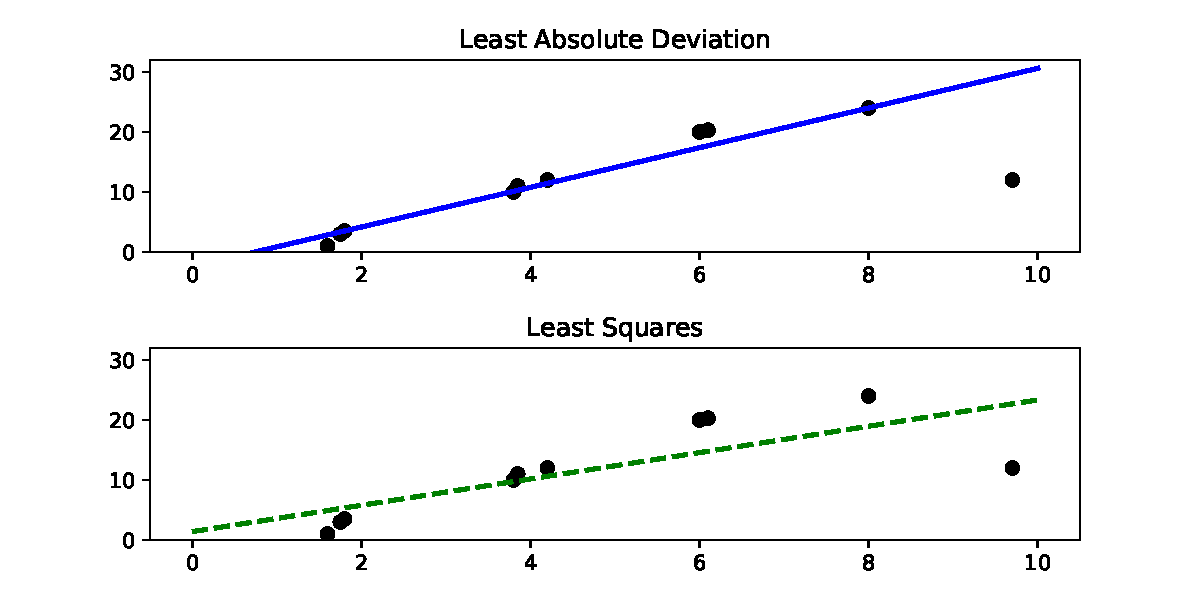
\includegraphics[width=\textwidth]{figures/leastAbsDev.pdf}
\caption{Fitted lines produced by least absolute deviations (top) and least squares (bottom). The presence of an outlier accounts for the
stark difference between the two lines.}
\label{fig:leastAbsDev}
\end{figure}

While least absolute deviations is robust with respect to outliers, small horizontal perturbations of the data points can lead to very different fitted lines.
Hence, the least absolute deviations solution is less stable than the least squares solution.
In some cases there are even infinitely many lines that minimize the least absolute deviations error term.
However, one can expect a unique solution in most cases.

The least absolute deviations solution arises naturally when we assume that the residual terms $\Beta\trp \mathbf{x}_i + b - y_i$ have a particular statistical distribution (the Laplace distribution).
Ultimately, however, the choice between least absolute deviations and least squares depends on the nature of the data at hand, as well as your own good judgment.

% =============================================================================
% =============================================================================
% EDITED TO HERE ==============================================================
% =============================================================================
% =============================================================================

\subsection*{LAD as a Linear Program}
We can formulate the least absolute deviations problem as a linear program, and then solve it using our interior point method.
For $i = 1, 2, \ldots, m$ we introduce the artificial variable $u_i$ to take the place of the error term $|\Beta\trp \mathbf{x}_i + b - y_i|$, and we require this variable to satisfy $u_i \geq |\Beta\trp \mathbf{x}_i + b - y_i|$.
This constraint is not yet linear, but we can split it into an equivalent set of two linear constraints:
\begin{align*}
u_i &\geq \Beta\trp \mathbf{x}_i + b - y_i,\\
u_i &\geq y_i - \Beta\trp \mathbf{x}_i - b.
\end{align*}
The $u_i$ are implicitly constrained to be nonnegative.

Our linear program can now be stated as follows:
\begin{align*}
\text{minimize }\qquad &\sum_{i=1}^m u_i\\
\text{subject to }\qquad &u_i \geq \Beta\trp \mathbf{x}_i + b - y_i,\\
&u_i \geq y_i - \Beta\trp \mathbf{x}_i - b.
\end{align*}
Now for each inequality constraint, we bring all variables ($u_i, \Beta, b$) to the left hand side and introduce a nonnegative slack variable to transform the constraint into an equality:
\begin{align*}
u_i  - \Beta\trp \mathbf{x}_i - b - s_{2i-1}&= -y_i,\\
u_i +\Beta\trp \mathbf{x}_i + b - s_{2i}&= y_i,\\
s_{2i-1}, s_{2i}&\geq 0.
\end{align*}

Notice that the variables $\Beta, b$ are not assumed to be nonnegative, but in our interior point method, all variables are assumed to be nonnegative.
We can fix this situation by writing these variables as the difference of nonnegative variables:
\begin{align*}
  \Beta &= \Beta_1 - \Beta_2,\\
  b &= b_1 - b_2,\\
  &\Beta_1, \Beta_2\succeq \0; b_1, b_2 \geq 0.
\end{align*}
Substituting these values into our constraints, we have the following system of constraints:
\begin{align*}
u_i  - \Beta_1\trp \mathbf{x}_i + \Beta_2\trp \mathbf{x}_i - b_1 + b_2 - s_{2i-1}&= -y_i,\\
u_i + \Beta_1\trp \mathbf{x}_i - \Beta_2\trp \mathbf{x}_i + b_1 - b_2 - s_{2i}&= y_i,\\
\Beta_1, \Beta_2 \succeq \0; u_i, b_1, b_2, s_{2i-1}, s_{2i}&\geq 0.
\end{align*}
Writing $\mathbf{y} = (-y_1, y_1, -y_2, y_2, \ldots, -y_m, y_m)\trp $ and $\Beta_i = (\beta_{i,1}, \ldots, \beta_{i,n})\trp $ for $i = \{1, 2\}$, we can aggregate all of our variables into one vector as follows:
\[
\mathbf{v} = (u_1,\ldots, u_m, \beta_{1,1},\ldots, \beta_{1,n}, \beta_{2,1},\ldots, \beta_{2,n}, b_1, b_2, s_1,\ldots,s_{2m})\trp .
\]
Defining $\c = (1, 1, \ldots, 1, 0, \ldots, 0)\trp $ (where only the first $m$ entries are equal to 1), we can write our objective function as
\[
\sum_{i=1}^m u_i = \mathbf{c}\trp \mathbf{v}.
\]
Hence, the final form of our linear program is:
\begin{align*}
  \text{minimize }\qquad &\mathbf{c}\trp \mathbf{v}\\
  \text{subject to }\qquad A\mathbf{v} &= \mathbf{y},\\
  \mathbf{v} &\succeq \0,
\end{align*}
where $A$ is a matrix containing the coefficients of the constraints.
Our constraints are now equalities, and the variables are all nonnegative, so we are ready to use our interior point method to obtain the solution.

\subsection*{LAD Example}

Consider the following example.
We start with an array \li{data}, each row of which consists of the values $y_i, x_{i,1},\ldots,x_{i,n}$, where $\mathbf{x}_i = (x_{i,1}, x_{i,2}, \ldots, x_{i,n})\trp $.
We will have $3m + 2(n+1)$ variables in our linear program.
Below, we initialize the vectors $\mathbf{c}$ and $\mathbf{y}$.
\begin{lstlisting}
>>> m = data.shape[0]
>>> n = data.shape[1] - 1
>>> c = np.zeros(3*m + 2*(n + 1))
>>> c[:m] = 1
>>> y = np.empty(2*m)
>>> y[::2] = -data[:, 0]
>>> y[1::2] = data[:, 0]
>>> x = data[:, 1:]
\end{lstlisting}

The hardest part is initializing the constraint matrix correctly.
It has $2m$ rows and $3m + 2(n+1)$ columns.
Try writing out the constraint matrix by hand for small $m, n$, and make sure you understand why the code below is correct.
% TODO: Do this with NumPy stacking.
\begin{lstlisting}
>>> A = np.ones((2*m, 3*m + 2*(n + 1)))
>>> A[::2, :m] = np.eye(m)
>>> A[1::2, :m] = np.eye(m)
>>> A[::2, m:m+n] = -x
>>> A[1::2, m:m+n] = x
>>> A[::2, m+n:m+2*n] = x
>>> A[1::2, m+n:m+2*n] = -x
>>> A[::2, m+2*n] = -1
>>> A[1::2, m+2*n+1] = -1
>>> A[:, m+2*n+2:] = -np.eye(2*m, 2*m)
\end{lstlisting}

Now we can calculate the solution by calling our interior point function.
\begin{lstlisting}
>>> sol = interiorPoint(A, y, c, niter=10)[0]
\end{lstlisting}

However, the variable \li{sol} holds the value for the vector
\[
\mathbf{v} = (u_1,\ldots, u_m, \beta_{1,1},\ldots, \beta_{1,n}, \beta_{2,1},\ldots, \beta_{2,n}, b_1, b_2, s_1,\ldots,s_{2m+1})\trp .
\]
We extract values of $\Beta = \Beta_1-\Beta_2$ and $b = b_1 - b_2$ with the following code:
\begin{lstlisting}
>>> beta = sol[m:m+n] - sol[m+n:m+2*n]
>>> b = sol[m+2*n] - sol[m+2*n+1]
\end{lstlisting}

\begin{problem} % Least Total Deviations Problem ------------------------------
The file \li{simdata.txt} contains two columns of data.
The first gives the values of the response variables ($y_i$), and the second column gives the values of the explanatory variables ($\x_i$).
Find the least absolute deviations line for this data set, and plot it together with the data.
Plot the least squares solution as well to compare the results.
\begin{lstlisting}
>>> from scipy.stats import linregress
>>> slope, intercept = linregress(data[:,1], data[:,0])[:2]
>>> domain = np.linspace(0,10,200)
>>> plt.plot(domain, domain*slope + intercept)
\end{lstlisting}
% \begin{figure}[H] % solution to the problem with new simdata.
% \centering
% \includegraphics[width=\textwidth]{figures/LADprob.pdf}
% \label{fig:LADprob}
% \end{figure}
\end{problem}
